
\input{../../2021/style/preamble4tex}
% dependencies: amsmath, amssymb, dsfont
% math spaces
\ifdefined\N
\renewcommand{\N}{\mathds{N}} % N, naturals
\else \newcommand{\N}{\mathds{N}} \fi
\newcommand{\Z}{\mathds{Z}} % Z, integers
\newcommand{\Q}{\mathds{Q}} % Q, rationals
\newcommand{\R}{\mathds{R}} % R, reals
\ifdefined\C
\renewcommand{\C}{\mathds{C}} % C, complex
\else \newcommand{\C}{\mathds{C}} \fi
\newcommand{\continuous}{\mathcal{C}} % C, space of continuous functions
\newcommand{\M}{\mathcal{M}} % machine numbers
\newcommand{\epsm}{\epsilon_m} % maximum error

% counting / finite sets
\newcommand{\setzo}{\{0, 1\}} % set 0, 1
\newcommand{\setmp}{\{-1, +1\}} % set -1, 1
\newcommand{\unitint}{[0, 1]} % unit interval

% basic math stuff
\newcommand{\xt}{\tilde x} % x tilde
\DeclareMathOperator*{\argmax}{arg\,max} % argmax
\DeclareMathOperator*{\argmin}{arg\,min} % argmin
\newcommand{\argminlim}{\mathop{\mathrm{arg\,min}}\limits} % argmax with limits
\newcommand{\argmaxlim}{\mathop{\mathrm{arg\,max}}\limits} % argmin with limits
\newcommand{\sign}{\operatorname{sign}} % sign, signum
\newcommand{\I}{\mathbb{I}} % I, indicator
\newcommand{\order}{\mathcal{O}} % O, order
\newcommand{\bigO}{\mathcal{O}} % Big-O Landau
\newcommand{\littleo}{{o}} % Little-o Landau
\newcommand{\pd}[2]{\frac{\partial{#1}}{\partial #2}} % partial derivative
\newcommand{\floorlr}[1]{\left\lfloor #1 \right\rfloor} % floor
\newcommand{\ceillr}[1]{\left\lceil #1 \right\rceil} % ceiling
\newcommand{\indep}{\perp \!\!\! \perp} % independence symbol

% sums and products
\newcommand{\sumin}{\sum\limits_{i=1}^n} % summation from i=1 to n
\newcommand{\sumim}{\sum\limits_{i=1}^m} % summation from i=1 to m
\newcommand{\sumjn}{\sum\limits_{j=1}^n} % summation from j=1 to p
\newcommand{\sumjp}{\sum\limits_{j=1}^p} % summation from j=1 to p
\newcommand{\sumik}{\sum\limits_{i=1}^k} % summation from i=1 to k
\newcommand{\sumkg}{\sum\limits_{k=1}^g} % summation from k=1 to g
\newcommand{\sumjg}{\sum\limits_{j=1}^g} % summation from j=1 to g
\newcommand{\meanin}{\frac{1}{n} \sum\limits_{i=1}^n} % mean from i=1 to n
\newcommand{\meanim}{\frac{1}{m} \sum\limits_{i=1}^m} % mean from i=1 to n
\newcommand{\meankg}{\frac{1}{g} \sum\limits_{k=1}^g} % mean from k=1 to g
\newcommand{\prodin}{\prod\limits_{i=1}^n} % product from i=1 to n
\newcommand{\prodkg}{\prod\limits_{k=1}^g} % product from k=1 to g
\newcommand{\prodjp}{\prod\limits_{j=1}^p} % product from j=1 to p

% linear algebra
\newcommand{\one}{\bm{1}} % 1, unitvector
\newcommand{\zero}{\mathbf{0}} % 0-vector
\newcommand{\id}{\bm{I}} % I, identity
\newcommand{\diag}{\operatorname{diag}} % diag, diagonal
\newcommand{\trace}{\operatorname{tr}} % tr, trace
\newcommand{\spn}{\operatorname{span}} % span
\newcommand{\scp}[2]{\left\langle #1, #2 \right\rangle} % <.,.>, scalarproduct
\newcommand{\mat}[1]{\begin{pmatrix} #1 \end{pmatrix}} % short pmatrix command
\newcommand{\Amat}{\mathbf{A}} % matrix A
\newcommand{\Deltab}{\mathbf{\Delta}} % error term for vectors

% basic probability + stats
\renewcommand{\P}{\mathds{P}} % P, probability
\newcommand{\E}{\mathds{E}} % E, expectation
\newcommand{\var}{\mathsf{Var}} % Var, variance
\newcommand{\cov}{\mathsf{Cov}} % Cov, covariance
\newcommand{\corr}{\mathsf{Corr}} % Corr, correlation
\newcommand{\normal}{\mathcal{N}} % N of the normal distribution
\newcommand{\iid}{\overset{i.i.d}{\sim}} % dist with i.i.d superscript
\newcommand{\distas}[1]{\overset{#1}{\sim}} % ... is distributed as ...

% machine learning
\newcommand{\Xspace}{\mathcal{X}} % X, input space
\newcommand{\Yspace}{\mathcal{Y}} % Y, output space
\newcommand{\Zspace}{\mathcal{Z}} % Z, space of sampled datapoints
\newcommand{\nset}{\{1, \ldots, n\}} % set from 1 to n
\newcommand{\pset}{\{1, \ldots, p\}} % set from 1 to p
\newcommand{\gset}{\{1, \ldots, g\}} % set from 1 to g
\newcommand{\Pxy}{\mathbb{P}_{xy}} % P_xy
\newcommand{\Exy}{\mathbb{E}_{xy}} % E_xy: Expectation over random variables xy
\newcommand{\xv}{\mathbf{x}} % vector x (bold)
\newcommand{\xtil}{\tilde{\mathbf{x}}} % vector x-tilde (bold)
\newcommand{\yv}{\mathbf{y}} % vector y (bold)
\newcommand{\xy}{(\xv, y)} % observation (x, y)
\newcommand{\xvec}{\left(x_1, \ldots, x_p\right)^\top} % (x1, ..., xp)
\newcommand{\Xmat}{\mathbf{X}} % Design matrix
\newcommand{\allDatasets}{\mathds{D}} % The set of all datasets
\newcommand{\allDatasetsn}{\mathds{D}_n}  % The set of all datasets of size n
\newcommand{\D}{\mathcal{D}} % D, data
\newcommand{\Dn}{\D_n} % D_n, data of size n
\newcommand{\Dtrain}{\mathcal{D}_{\text{train}}} % D_train, training set
\newcommand{\Dtest}{\mathcal{D}_{\text{test}}} % D_test, test set
\newcommand{\xyi}[1][i]{\left(\xv^{(#1)}, y^{(#1)}\right)} % (x^i, y^i), i-th observation
\newcommand{\Dset}{\left( \xyi[1], \ldots, \xyi[n]\right)} % {(x1,y1)), ..., (xn,yn)}, data
\newcommand{\defAllDatasetsn}{(\Xspace \times \Yspace)^n} % Def. of the set of all datasets of size n
\newcommand{\defAllDatasets}{\bigcup_{n \in \N}(\Xspace \times \Yspace)^n} % Def. of the set of all datasets
\newcommand{\xdat}{\left\{ \xv^{(1)}, \ldots, \xv^{(n)}\right\}} % {x1, ..., xn}, input data
\newcommand{\ydat}{\left\{ \yv^{(1)}, \ldots, \yv^{(n)}\right\}} % {y1, ..., yn}, input data
\newcommand{\yvec}{\left(y^{(1)}, \hdots, y^{(n)}\right)^\top} % (y1, ..., yn), vector of outcomes
\newcommand{\greekxi}{\xi} % Greek letter xi
\renewcommand{\xi}[1][i]{\xv^{(#1)}} % x^i, i-th observed value of x
\newcommand{\yi}[1][i]{y^{(#1)}} % y^i, i-th observed value of y
\newcommand{\xivec}{\left(x^{(i)}_1, \ldots, x^{(i)}_p\right)^\top} % (x1^i, ..., xp^i), i-th observation vector
\newcommand{\xj}{\xv_j} % x_j, j-th feature
\newcommand{\xjvec}{\left(x^{(1)}_j, \ldots, x^{(n)}_j\right)^\top} % (x^1_j, ..., x^n_j), j-th feature vector
\newcommand{\phiv}{\mathbf{\phi}} % Basis transformation function phi
\newcommand{\phixi}{\mathbf{\phi}^{(i)}} % Basis transformation of xi: phi^i := phi(xi)

%%%%%% ml - models general
\newcommand{\lamv}{\bm{\lambda}} % lambda vector, hyperconfiguration vector
\newcommand{\Lam}{\bm{\Lambda}}	 % Lambda, space of all hpos
% Inducer / Inducing algorithm
\newcommand{\preimageInducer}{\left(\defAllDatasets\right)\times\Lam} % Set of all datasets times the hyperparameter space
\newcommand{\preimageInducerShort}{\allDatasets\times\Lam} % Set of all datasets times the hyperparameter space
% Inducer / Inducing algorithm
\newcommand{\ind}{\mathcal{I}} % Inducer, inducing algorithm, learning algorithm

% continuous prediction function f
\newcommand{\ftrue}{f_{\text{true}}}  % True underlying function (if a statistical model is assumed)
\newcommand{\ftruex}{\ftrue(\xv)} % True underlying function (if a statistical model is assumed)
\newcommand{\fx}{f(\xv)} % f(x), continuous prediction function
\newcommand{\fdomains}{f: \Xspace \rightarrow \R^g} % f with domain and co-domain
\newcommand{\Hspace}{\mathcal{H}} % hypothesis space where f is from
\newcommand{\fbayes}{f^{\ast}} % Bayes-optimal model
\newcommand{\fxbayes}{f^{\ast}(\xv)} % Bayes-optimal model
\newcommand{\fkx}[1][k]{f_{#1}(\xv)} % f_j(x), discriminant component function
\newcommand{\fh}{\hat{f}} % f hat, estimated prediction function
\newcommand{\fxh}{\fh(\xv)} % fhat(x)
\newcommand{\fxt}{f(\xv ~|~ \thetav)} % f(x | theta)
\newcommand{\fxi}{f\left(\xv^{(i)}\right)} % f(x^(i))
\newcommand{\fxih}{\hat{f}\left(\xv^{(i)}\right)} % f(x^(i))
\newcommand{\fxit}{f\left(\xv^{(i)} ~|~ \thetav\right)} % f(x^(i) | theta)
\newcommand{\fhD}{\fh_{\D}} % fhat_D, estimate of f based on D
\newcommand{\fhDtrain}{\fh_{\Dtrain}} % fhat_Dtrain, estimate of f based on D
\newcommand{\fhDnlam}{\fh_{\Dn, \lamv}} %model learned on Dn with hp lambda
\newcommand{\fhDlam}{\fh_{\D, \lamv}} %model learned on D with hp lambda
\newcommand{\fhDnlams}{\fh_{\Dn, \lamv^\ast}} %model learned on Dn with optimal hp lambda
\newcommand{\fhDlams}{\fh_{\D, \lamv^\ast}} %model learned on D with optimal hp lambda

% discrete prediction function h
\newcommand{\hx}{h(\xv)} % h(x), discrete prediction function
\newcommand{\hh}{\hat{h}} % h hat
\newcommand{\hxh}{\hat{h}(\xv)} % hhat(x)
\newcommand{\hxt}{h(\xv | \thetav)} % h(x | theta)
\newcommand{\hxi}{h\left(\xi\right)} % h(x^(i))
\newcommand{\hxit}{h\left(\xi ~|~ \thetav\right)} % h(x^(i) | theta)
\newcommand{\hbayes}{h^{\ast}} % Bayes-optimal classification model
\newcommand{\hxbayes}{h^{\ast}(\xv)} % Bayes-optimal classification model

% yhat
\newcommand{\yh}{\hat{y}} % yhat for prediction of target
\newcommand{\yih}{\hat{y}^{(i)}} % yhat^(i) for prediction of ith targiet
\newcommand{\resi}{\yi- \yih}

% theta
\newcommand{\thetah}{\hat{\theta}} % theta hat
\newcommand{\thetav}{\bm{\theta}} % theta vector
\newcommand{\thetavh}{\bm{\hat\theta}} % theta vector hat
\newcommand{\thetat}[1][t]{\thetav^{[#1]}} % theta^[t] in optimization
\newcommand{\thetatn}[1][t]{\thetav^{[#1 +1]}} % theta^[t+1] in optimization
\newcommand{\thetahDnlam}{\thetavh_{\Dn, \lamv}} %theta learned on Dn with hp lambda
\newcommand{\thetahDlam}{\thetavh_{\D, \lamv}} %theta learned on D with hp lambda
\newcommand{\mint}{\min_{\thetav \in \Theta}} % min problem theta
\newcommand{\argmint}{\argmin_{\thetav \in \Theta}} % argmin theta

% densities + probabilities
% pdf of x
\newcommand{\pdf}{p} % p
\newcommand{\pdfx}{p(\xv)} % p(x)
\newcommand{\pixt}{\pi(\xv~|~ \thetav)} % pi(x|theta), pdf of x given theta
\newcommand{\pixit}[1][i]{\pi\left(\xi[#1] ~|~ \thetav\right)} % pi(x^i|theta), pdf of x given theta
\newcommand{\pixii}[1][i]{\pi\left(\xi[#1]\right)} % pi(x^i), pdf of i-th x

% pdf of (x, y)
\newcommand{\pdfxy}{p(\xv,y)} % p(x, y)
\newcommand{\pdfxyt}{p(\xv, y ~|~ \thetav)} % p(x, y | theta)
\newcommand{\pdfxyit}{p\left(\xi, \yi ~|~ \thetav\right)} % p(x^(i), y^(i) | theta)

% pdf of x given y
\newcommand{\pdfxyk}[1][k]{p(\xv | y= #1)} % p(x | y = k)
\newcommand{\lpdfxyk}[1][k]{\log p(\xv | y= #1)} % log p(x | y = k)
\newcommand{\pdfxiyk}[1][k]{p\left(\xi | y= #1 \right)} % p(x^i | y = k)

% prior probabilities
\newcommand{\pik}[1][k]{\pi_{#1}} % pi_k, prior
\newcommand{\lpik}[1][k]{\log \pi_{#1}} % log pi_k, log of the prior
\newcommand{\pit}{\pi(\thetav)} % Prior probability of parameter theta

% posterior probabilities
\newcommand{\post}{\P(y = 1 ~|~ \xv)} % P(y = 1 | x), post. prob for y=1
\newcommand{\postk}[1][k]{\P(y = #1 ~|~ \xv)} % P(y = k | y), post. prob for y=k
\newcommand{\pidomains}{\pi: \Xspace \rightarrow \unitint} % pi with domain and co-domain
\newcommand{\pibayes}{\pi^{\ast}} % Bayes-optimal classification model
\newcommand{\pixbayes}{\pi^{\ast}(\xv)} % Bayes-optimal classification model
\newcommand{\pix}{\pi(\xv)} % pi(x), P(y = 1 | x)
\newcommand{\piv}{\bm{\pi}} % pi, bold, as vector
\newcommand{\pikx}[1][k]{\pi_{#1}(\xv)} % pi_k(x), P(y = k | x)
\newcommand{\pikxt}[1][k]{\pi_{#1}(\xv ~|~ \thetav)} % pi_k(x | theta), P(y = k | x, theta)
\newcommand{\pixh}{\hat \pi(\xv)} % pi(x) hat, P(y = 1 | x) hat
\newcommand{\pikxh}[1][k]{\hat \pi_{#1}(\xv)} % pi_k(x) hat, P(y = k | x) hat
\newcommand{\pixih}{\hat \pi(\xi)} % pi(x^(i)) with hat
\newcommand{\pikxih}[1][k]{\hat \pi_{#1}(\xi)} % pi_k(x^(i)) with hat
\newcommand{\pdfygxt}{p(y ~|~\xv, \thetav)} % p(y | x, theta)
\newcommand{\pdfyigxit}{p\left(\yi ~|~\xi, \thetav\right)} % p(y^i |x^i, theta)
\newcommand{\lpdfygxt}{\log \pdfygxt } % log p(y | x, theta)
\newcommand{\lpdfyigxit}{\log \pdfyigxit} % log p(y^i |x^i, theta)

% probababilistic
\newcommand{\bayesrulek}[1][k]{\frac{\P(\xv | y= #1) \P(y= #1)}{\P(\xv)}} % Bayes rule
\newcommand{\muk}{\bm{\mu_k}} % mean vector of class-k Gaussian (discr analysis)

% residual and margin
\newcommand{\eps}{\epsilon} % residual, stochastic
\newcommand{\epsv}{\bm{\epsilon}} % residual, stochastic, as vector
\newcommand{\epsi}{\epsilon^{(i)}} % epsilon^i, residual, stochastic
\newcommand{\epsh}{\hat{\epsilon}} % residual, estimated
\newcommand{\epsvh}{\hat{\epsv}} % residual, estimated, vector
\newcommand{\yf}{y \fx} % y f(x), margin
\newcommand{\yfi}{\yi \fxi} % y^i f(x^i), margin
\newcommand{\Sigmah}{\hat \Sigma} % estimated covariance matrix
\newcommand{\Sigmahj}{\hat \Sigma_j} % estimated covariance matrix for the j-th class

% ml - loss, risk, likelihood
\newcommand{\Lyf}{L\left(y, f\right)} % L(y, f), loss function
\newcommand{\Lypi}{L\left(y, \pi\right)} % L(y, pi), loss function
\newcommand{\Lxy}{L\left(y, \fx\right)} % L(y, f(x)), loss function
\newcommand{\Lxyi}{L\left(\yi, \fxi\right)} % loss of observation
\newcommand{\Lxyt}{L\left(y, \fxt\right)} % loss with f parameterized
\newcommand{\Lxyit}{L\left(\yi, \fxit\right)} % loss of observation with f parameterized
\newcommand{\Lxym}{L\left(\yi, f\left(\bm{\tilde{x}}^{(i)} ~|~ \thetav\right)\right)} % loss of observation with f parameterized
\newcommand{\Lpixy}{L\left(y, \pix\right)} % loss in classification
\newcommand{\Lpiv}{L\left(y, \piv\right)} % loss in classification
\newcommand{\Lpixyi}{L\left(\yi, \pixii\right)} % loss of observation in classification
\newcommand{\Lpixyt}{L\left(y, \pixt\right)} % loss with pi parameterized
\newcommand{\Lpixyit}{L\left(\yi, \pixit\right)} % loss of observation with pi parameterized
\newcommand{\Lhxy}{L\left(y, \hx\right)} % L(y, h(x)), loss function on discrete classes
\newcommand{\Lr}{L\left(r\right)} % L(r), loss defined on residual (reg) / margin (classif)
\newcommand{\lone}{|y - \fx|} % L1 loss
\newcommand{\ltwo}{\left(y - \fx\right)^2} % L2 loss
\newcommand{\lbernoullimp}{\ln(1 + \exp(-y \cdot \fx))} % Bernoulli loss for -1, +1 encoding
\newcommand{\lbernoullizo}{- y \cdot \fx + \log(1 + \exp(\fx))} % Bernoulli loss for 0, 1 encoding
\newcommand{\lcrossent}{- y \log \left(\pix\right) - (1 - y) \log \left(1 - \pix\right)} % cross-entropy loss
\newcommand{\lbrier}{\left(\pix - y \right)^2} % Brier score
\newcommand{\risk}{\mathcal{R}} % R, risk
\newcommand{\riskbayes}{\mathcal{R}^\ast}
\newcommand{\riskf}{\risk(f)} % R(f), risk
\newcommand{\riskdef}{\E_{y|\xv}\left(\Lxy \right)} % risk def (expected loss)
\newcommand{\riskt}{\mathcal{R}(\thetav)} % R(theta), risk
\newcommand{\riske}{\mathcal{R}_{\text{emp}}} % R_emp, empirical risk w/o factor 1 / n
\newcommand{\riskeb}{\bar{\mathcal{R}}_{\text{emp}}} % R_emp, empirical risk w/ factor 1 / n
\newcommand{\riskef}{\riske(f)} % R_emp(f)
\newcommand{\risket}{\mathcal{R}_{\text{emp}}(\thetav)} % R_emp(theta)
\newcommand{\riskr}{\mathcal{R}_{\text{reg}}} % R_reg, regularized risk
\newcommand{\riskrt}{\mathcal{R}_{\text{reg}}(\thetav)} % R_reg(theta)
\newcommand{\riskrf}{\riskr(f)} % R_reg(f)
\newcommand{\riskrth}{\hat{\mathcal{R}}_{\text{reg}}(\thetav)} % hat R_reg(theta)
\newcommand{\risketh}{\hat{\mathcal{R}}_{\text{emp}}(\thetav)} % hat R_emp(theta)
\newcommand{\LL}{\mathcal{L}} % L, likelihood
\newcommand{\LLt}{\mathcal{L}(\thetav)} % L(theta), likelihood
\newcommand{\LLtx}{\mathcal{L}(\thetav | \xv)} % L(theta|x), likelihood
\newcommand{\logl}{\ell} % l, log-likelihood
\newcommand{\loglt}{\logl(\thetav)} % l(theta), log-likelihood
\newcommand{\logltx}{\logl(\thetav | \xv)} % l(theta|x), log-likelihood
\newcommand{\errtrain}{\text{err}_{\text{train}}} % training error
\newcommand{\errtest}{\text{err}_{\text{test}}} % test error
\newcommand{\errexp}{\overline{\text{err}_{\text{test}}}} % avg training error

% lm
\newcommand{\thx}{\thetav^\top \xv} % linear model
\newcommand{\olsest}{(\Xmat^\top \Xmat)^{-1} \Xmat^\top \yv} % OLS estimator in LM

\input{../../latex-math/ml-bagging.tex}
\input{../../latex-math/ml-boosting.tex}
% ml - trees, extra trees

\newcommand{\Np}{\mathcal{N}} % (Parent) node N
\newcommand{\Npk}{\Np_k} % node N_k
\newcommand{\Nl}{\Np_1}	% Left node N_1
\newcommand{\Nr}{\Np_2} % Right node N_2
\newcommand{\pikN}[1][k]{\pi_#1^{(\Np)}} % class probability node N
\newcommand{\pikNh}[1][k]{\hat\pi_#1^{(\Np)}} % estimated class probability node N
\newcommand{\pikNlh}[1][k]{\hat\pi_#1^{(\Nl)}} % estimated class probability left node
\newcommand{\pikNrh}[1][k]{\hat\pi_#1^{(\Nr)}} % estimated class probability right node


\begin{document}

\lecturechapter{11}{XGBoost}
\lecture{Fortgeschrittene Computerintensive Methoden}

% sources: https://homes.cs.washington.edu/~tqchen/pdf/BoostedTree.pdf
% sources: https://towardsdatascience.com/boosting-algorithm-xgboost-4d9ec0207d
% sources: https://devblogs.nvidia.com/parallelforall/gradient-boosting-decision-trees-xgboost-cuda/

\begin{vbframe}{Motivation}

\textbf{Chen and Guestrin (2016)}:

\pkg{XGBoost} (short for eXtreme Gradient Boosting) is an open-source software
library with R/Python/Julia/Spark interface.

\lz

A scalable regularized tree boosting system:
\begin{itemize}
  \item Efficient implementation in \emph{C++}.
  \item Parallel (approximate) split finding.
  \item Handling of \emph{sparse data}.
  \item Support of cluster-computing frameworks.
\end{itemize}

\lz

State-of-the-art machine learning method:
\begin{itemize}
  \item Many winning solutions at Kaggle use XGBoost.
  \item KDDCup 2015 Top 10 used XGBoost.
\end{itemize}

\end{vbframe}

\begin{vbframe}{Loss minimization}

\pkg{XGBoost} uses a risk function with 3 regularization terms:
\vskip -1em
\begin{multline*}
  \riskr^{[m]} = \sum_{i=1}^{n} L\left(\yi, \fmd(\xi) + \bmm(\xi)\right)\\
   + \gamma J_1(\bmm) + \lambda J_2(\bmm) + \alpha J_3(\bmm),
\end{multline*}


with $J_1(\bmm) = T^{[m]}$ to regularize tree depth, where $T^{[m]}$ is the number of leaves in the tree.

\lz

$J_2(\bmm) = \left\|\mathbf{c}^{[m]}\right\|^2_2$ and $J_3(\bmm) = \left\|\mathbf{c}^{[m]}\right\|_1$ are $L2$ and $L1$ regularizers of the terminal region scores $c_t^{[m]}, t=1,\dots,T^{[m]}$.

\lz

\textbf{Note:} In the following we define $J(\bmm) := \gamma J_1(\bmm) + \lambda J_2(\bmm) + \alpha J_3(\bmm)$ to simplify the notation.

\framebreak

Recall the way a tree base learner $\bmm(\xv)$ can be fitted loss-optimally in gradient boosting:

$$
\tilde{\mathbf{c}}^{[m]} = \argmin_{(c_1,\dots,c_{T^{[m]}})}\sum_{i = 1}^n L(\yi, \fmd(\xi) + \bmm(\xi, c_1,\dots,c_{T^{[m]}})).
$$

The direction of steepest descent for the update is then

$$
-\frac{\partial L(y, \fmd(\xv) + \bmm(\xv))}{\partial \bmm(\xv)}
$$

for each $\xi, i = 1,\dots, n$.

\lz

\textbf{Note:} $J(\bmm)$ is omitted for now but will be re-introduced later.

\framebreak

To approximate the loss in iteration $m$, use a second-order Taylor expansion around $\fmd(\xv)$:
\vskip  -1em
\begin{align*}
  &L(y, \fmd(\xv) + \bmm(\xv)) \approx \\
  &\qquad L(y, \fmd(\xv)) + g^{[m]}(\xv)\bmm(\xv) + \frac12 h^{[m]}(\xv)\bmm(\xv)^2,
\end{align*}

with gradient

$$
g^{[m]}(\xv) = \frac{\partial L(y, \fmd(\xv))}{\partial \fmd(\xv)}
$$

and Hessian

$$
h^{[m]}(\xv) = \frac{\partial^2 L(y, \fmd(\xv))}{\partial {\fmd(\xv)}^2}.
$$

\textbf{Note:} $g^{[m]}(\xv)$ are the negative pseudo-residuals $-\rmm$ we use in standard gradient boosting to determine the direction of the update.

\framebreak

Since $L(y, \fmd(\xv))$ is a constant, the optimization criterion simplifies to

\begin{align*}
\riskr^{[m]} \approx &\sum_{i = 1}^n g^{[m]}(\xi)\bmm(\xi) + \frac12 h^{[m]}(\xi)\bmm(\xi)^2 + J(\bmm) + const\\
\propto&\sum_{t=1}^{T^{[m]}}\sum_{\xi\in R_t^{[m]}} g^{[m]}(\xi)c^{[m]}_t + \frac12 h^{[m]}(\xi)(c^{[m]}_t)^2 + J(\bmm).\intertext{Defining $G^{[m]}_t$ and $H^{[m]}_t$ as the sum of the gradients and Hessians, respectively, in terminal node $t$ yields
}
=& \sum_{t=1}^{T^{[m]}}G^{[m]}_t c^{[m]}_t+\frac12 H^{[m]}_t (c^{[m]}_t)^2 + J(\bmm).
\end{align*}



\framebreak

Expanding $J(\bmm)$, we get
\begin{align*}
\riskr^{[m]} = &\sum_{t=1}^{T^{[m]}}\left(G^{[m]}_t c^{[m]}_t+\frac12 H^{[m]}_t (c^{[m]}_t)^2 + \frac12\lambda(c^{[m]}_t)^2 + \alpha |c^{[m]}_t|\right) + \gamma T^{[m]}\\
=&\sum_{t=1}^{T^{[m]}}\left(G^{[m]}_t c^{[m]}_t+\frac12 (H^{[m]}_t + \lambda) (c^{[m]}_t)^2 + \alpha |c_t^{[m]}|\right) + \gamma T^{[m]}.
\end{align*}

\lz

\textbf{Note:} The factor $\frac12$ is added to the $L2$ regularization to simplify the notation as shown in the second step.
This does not impact estimation since we can just define $\lambda = 2\tilde\lambda$.

\framebreak

Since

$$
\frac{\partial \riskr^{[m]}}{\partial c^{[m]}_t} =
\begin{cases}
  (G^{[m]}_t - \alpha) + (H^{[m]}_t + \lambda) c^{m}_t &\text{ for } c^{m}_t < 0 \\
  (G^{[m]}_t + \alpha) + (H^{[m]}_t + \lambda) c^{m}_t &\text{ for } c^{m}_t > 0, \\
\end{cases}
$$

the optimal weights $\tilde{c}^{[m]}_1,\dots, \tilde{c}^{[m]}_{T^{[m]}}$ can then be calculated as

\lz
$$
\tilde{c}^{[m]}_t = - \frac{t_\alpha\left(G^{[m]}_t\right)}{H^{[m]}_t + \lambda}, t=1,\dots T^{[m]},
$$
with $$t_\alpha(x) = \begin{cases}
  x - \alpha &\text{ for } x > \alpha \\
  x + \alpha &\text{ for } x < - \alpha \\
  0  &\text{ for } |x| \leq \alpha.
\end{cases}$$

\end{vbframe}

\begin{vbframe}{Loss minimization - split finding}

To evaluate the performance of a candidate split that divides the instances in region $R_t^{[m]}$ into a left and right node we use the \textbf{risk reduction} achieved by that split:
$$
\tilde S_{LR} =
 \frac12 \left[\frac{t_\alpha\left(G^{[m]}_{tL}\right)^2}{H^{[m]}_{tL} + \lambda} + \frac{t_\alpha\left(G^{[m]}_{tR}\right)^2}{H^{[m]}_{tR} + \lambda} - \frac{t_\alpha\left(G^{[m]}_{t}\right)^2}{H^{[m]}_{t} + \lambda}\right] - \gamma,
$$
where the subscripts $L$ and $R$ denote the left and right leaves after the split.

% derivation for this: write out change in loss function, case distinction acording to sign of t_a(G)/(H + lambda)

\lz

\framebreak

\begin{algorithm}[H]

\begin{footnotesize}
\begin{center}

  \begin{algorithmic}[1]
    \State \textbf{Input} $I$: \emph{instance set of current node}
    \State \textbf{Input} $p$: \emph{dimension of feature space}
    \State $gain \gets 0$
    \State $G \gets \sum_{i \in I} g(\xi), {H} \gets \sum_{i \in I} h(\xi)$
    \For{$j = 1 \to p$}
      \State $G_L \gets 0, {H}_L \gets 0$
      \For{$i$ in sorted($I$, by $x_{j}$)}
        \State ${G}_L \gets {G}_L + g(\xi), {H}_L \gets {H}_L + h(\xi)$
        \State ${G}_R \gets G - {G}_L, {H}_R \gets {H} - {H}_L$
        \State compute $\tilde S_{LR}$
      \EndFor
    \EndFor
    \State \textbf{Output} Split with maximal $\tilde S_{LR}$
  \end{algorithmic}
\end{center}
\end{footnotesize}
\caption{(Exact) Algorithm for split finding}
\end{algorithm}

\end{vbframe}

\begin{vbframe}{Approximate split-finding algorithms}

Three different algorithms to search for these splits are implemented in XGBoost.

\lz

\begin{itemize}
\item[] The \textbf{exact greedy algorithm} iterates over all possible splits of all features.
\lz
\item[] The \textbf{global approximate algorithm} iterates over percentiles of the empirical distribution of each feature.
\lz
\item[] The \textbf{local approximate algorithm} does the same as the global, but recalculates the percentiles after each split.
\end{itemize}

\framebreak

\begin{algorithm}[H]
\begin{footnotesize}
\begin{center}
  \begin{algorithmic}[1]
    \For{$j = 1 \to p$}
      \State Define possible split proposals $S_j = \{s_{j}^{(1)}, s_{j}^{(2)}, \hdots, s_{j}^{(l)}\}$ by percentiles on feature $j$.
      \State Proposal can be done once per tree (global), or in each node (local).
    \EndFor
    \For{$j = 1 \to p$}
      \State ${G}_{kv} \gets \sum_{i \in \{i|s_j^{(v)} \geq x_j^{(i)} > s_{k}^{(v - 1)}\}} g(\xi)$
      \State ${H}_{kv} \gets \sum_{i \in \{i|s_j^{(v)} \geq x_j^{(i)} > s_{k}^{(v - 1)}\}} h(\xi)$
    \EndFor
    \State Follow same steps as exact algorithm to find max score only among proposed splits.
  \end{algorithmic}
\end{center}
\end{footnotesize}
\caption{Approximate algorithm for split finding}
\end{algorithm}

\framebreak

\vspace{0.2cm}

\begin{center}
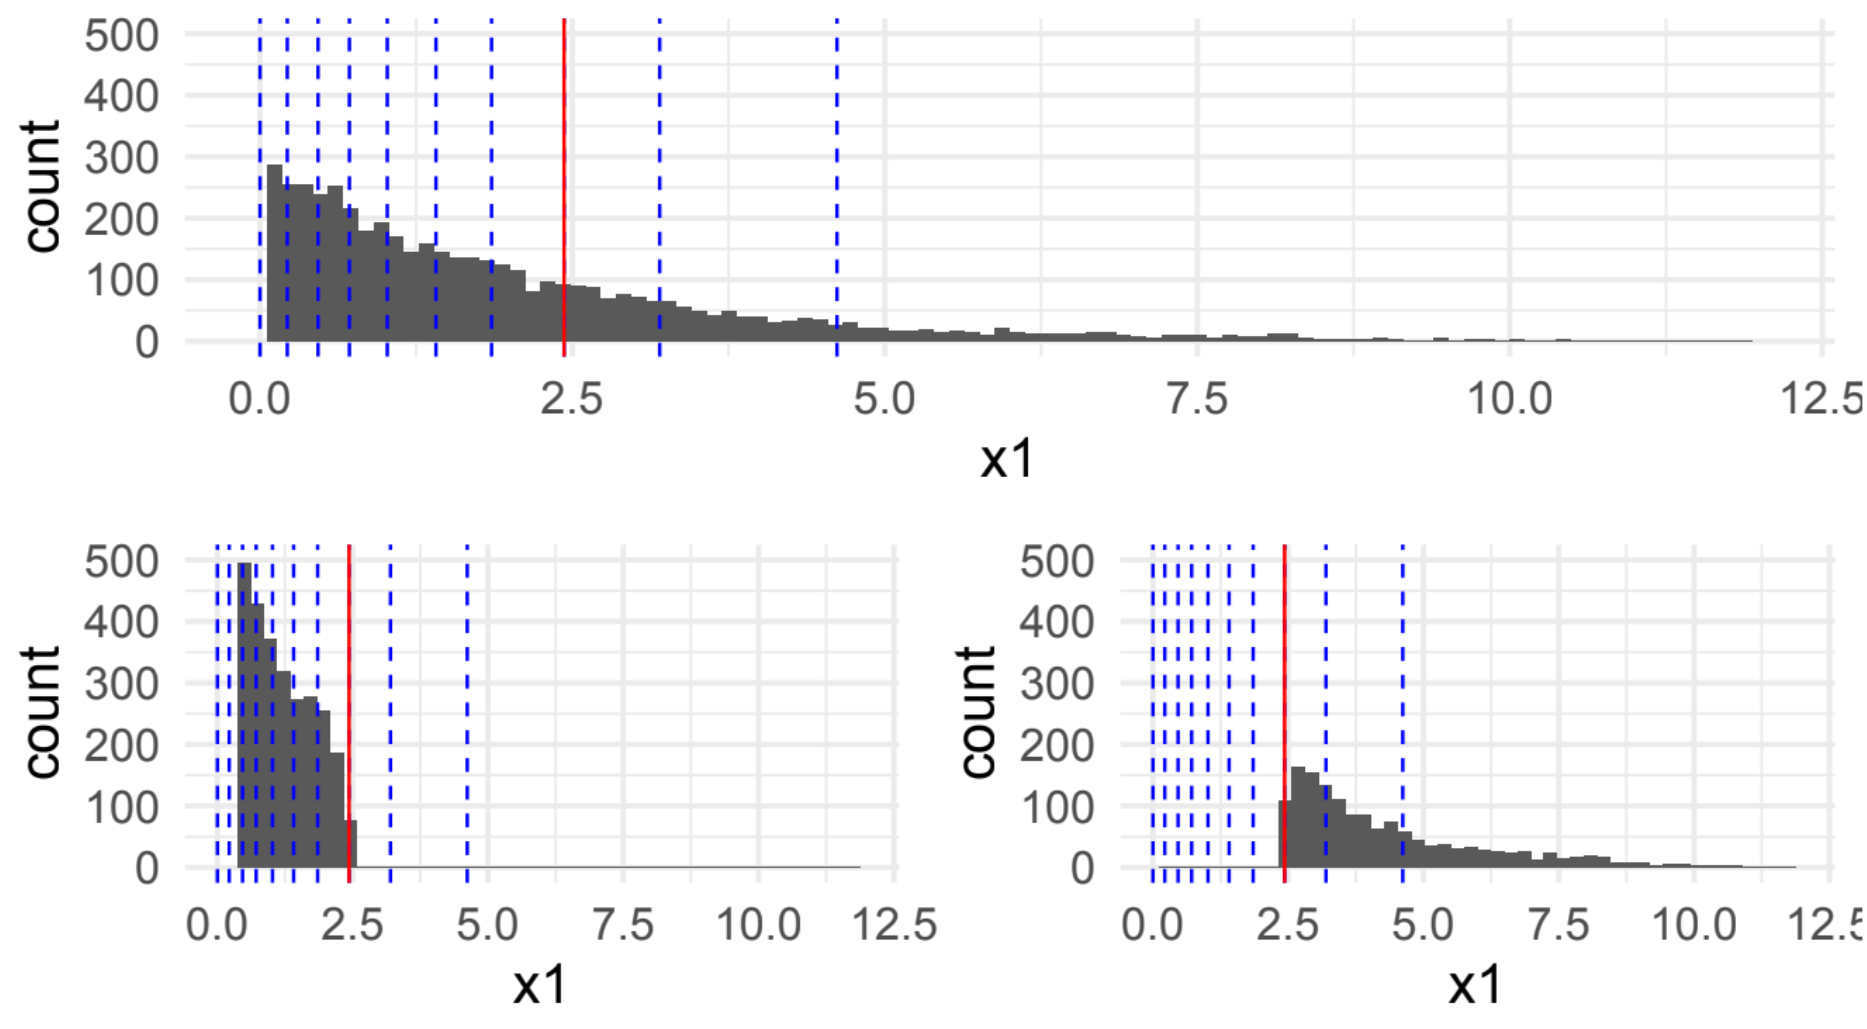
\includegraphics[width=0.9\textwidth]{figure_man/split-finding01.png}
\end{center}

Approximate \textbf{global} split finding.\\
Blue lines indicate percentiles, red line is the chosen split.
Proposals are not recomputed, allowing the right node only two possibilities.

\framebreak

\vspace{0.2cm}

\begin{center}
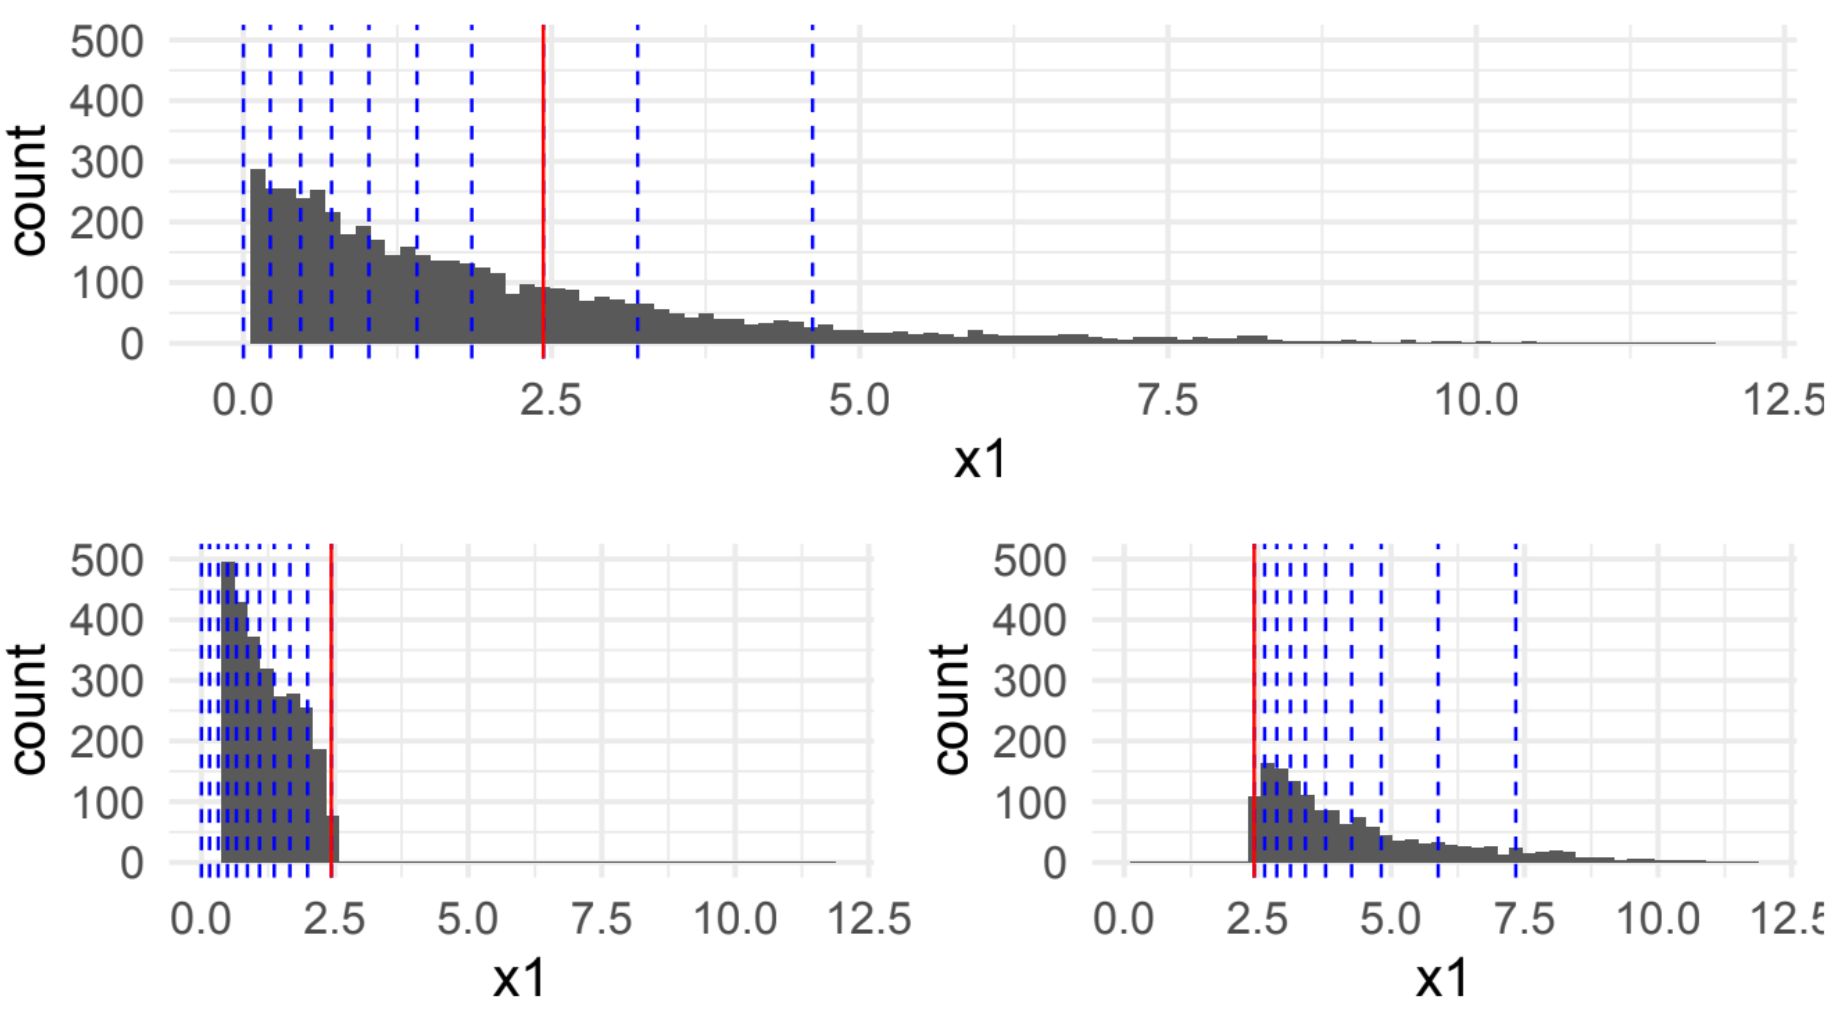
\includegraphics[width=0.9\textwidth]{figure_man/split-finding02.png}
\end{center}

Approximate \textbf{local} split finding.\\
Blue lines indicate percentiles, red line is the chosen split.
Percentiles are recalculated after each split.

\framebreak

Both approximate splitting algorithms are useful for large datasets as iteration over all splits becomes very expensive.

\lz

XGBoost also allows for sparsity-aware split finding, which means that for a large number of zero (or missing) values, a default direction in each node is introduced.

\lz

The calculation of the percentiles in the feature distributions can be parallelized, allowing parallel split finding for the approximate algorithms.

\end{vbframe}

\begin{vbframe}{Even more regularization}

Besides the regularization terms discussed above, XGBoost also incorporates a step length $\nu$ for the updates.

\lz

Furthermore, it uses \textbf{feature subsampling} similar to the random forest. Only a random subset of all features is considered for each split.

\lz

Stochastic gradient boosting, as introduced before, is utilized as well,
which means that in each iteration only a subset of the observations is used.

\lz

A final possibility for regularization is DART (Dropout Additive Regression Trees).
For each iteration only a fraction of previously fitted trees is considered.
After an update the joint contribution of the dropped tree and the tree new to the ensemble are scaled to avoid overshooting.

\end{vbframe}

\begin{vbframe}{Storage and out-of-memory calculation}

The data is stored in \textbf{blocks.}
Each of these blocks is stored in a compressed column format.

\lz

Depending on the split finding algorithm, these blocks contain the complete (sorted) data, or subsets of rows.

\lz

These blocks can be stored out-of-memory (on disk) to save memory and distributed across multiple machines for parallel computations.

\lz

For more details on this see \emph{Chen and Guestrin (2016)}.

\end{vbframe}

\begin{vbframe}{Summary}

XGBoost is an extremely powerful method, but also hard to configure correctly.
Overall, eight hyperparameters have to be set, which is difficult to do in practice and almost always requires tuning.

\lz

Different split finding algorithms can be selected, which allows XGBoost to be efficient even on very large datasets.

\lz

A large number of different regularization strategies is included to prevent overfitting.


\end{vbframe}

\begin{vbframe}{Comparison of major boosting systems}

\begin{tiny}
\begin{table}[]
\centering
\begin{tabular}{l|c|c|c|c|c|c}
System       & Exact algo. & Approx. algo. & Sparsity-aware & Variable importance & Parallel & Language   \\
\hline
ada          & yes         & no            & no             & no                  & no       & R          \\
GBM          & yes         & no            & partially      & yes                 & no       & R          \\
mboost       & yes         & no            & no             & no                  & no       & R          \\
compboost    & yes         & no            & yes            & yes                 & yes      & R          \\
H2O          & no          & yes           & partially      & yes                 & yes      & R (Java)   \\
XGBoost      & yes         & yes           & yes            & yes                 & yes      & R + Python \\
lightGBM     & no          & yes           & yes            & yes                 & yes      & R + Python \\
catboost     & no          & yes           & no             & yes                 & yes      & R + Python \\
scikit-learn & yes         & no            & no             & yes                 & no       & Python     \\
pGBRT        & no          & no            & no             & no                  & yes      & Python     \\
Spark MLLib  & no          & yes           & partially      & yes                 & yes      & R, Python, \\
             &             &               &                &                     &          & Java, Scala\\

\end{tabular}
\label{my-label}
\end{table}
\end{tiny}

\lz

\textbf{Note:} H2O is a commercial software written in Java with a solid R interface.
In the free version only two CPUs can be used.

%\framebreak
%
%We compare the performance in terms of accuray and runtime on five example data sets from OpenML.
%
%\lz
%
%All boosting algorithms use $100$ iterations, a learning rate of $0.1$ and a maximum tree depth of $4$ (except for mboost which uses linear models as base-learner).
%
%\lz
%
%We also compare to a random forest as a base-line.
%
%\framebreak
%<<echo=FALSE, fig.height=5>>=
%load("rsrc/benchmark.RData")
%plotBMRBoxplots(bmr, facet.wrap.ncol = 4)
%plotBMRBoxplots(bmr, measure = timetrain, facet.wrap.ncol = 4)
%@

%\framebreak

%Overall XGBoost performs well and is on par with commercial software like H2O.

%\lz

%The random forest is hard to beat in this benchmark. This is due to the fact that we did not do any tuning of the boosting hyperparameters.
%While this is quite important for boosting algorithms, a random forest is not as sensitive to its hyperparameters.

%\lz

%mboost with boosted linear models is overall worse than the other algorithms, but has the advantage of better interpretability.

\end{vbframe}

\endlecture
\end{document}

